\documentclass[12pt, a4paper]{article}
\usepackage[swedish]{babel}
\usepackage[version=4]{mhchem}
\usepackage{amsmath}
\usepackage[swedish]{varioref}
\usepackage{hyperref}
\hypersetup{
    colorlinks=true,
    linkcolor=black,
    pdftitle={Fysik 1 Uppslagverk},
    pdfpagemode=FullScreen
}
\usepackage[swedish]{cleveref}
\usepackage{amsthm}
\renewcommand\qedsymbol{V.S.V.}
\theoremstyle{definition}
\newtheorem{exm}{Exempel}
\usepackage{cancel}
\usepackage{float}
\usepackage{array}
\usepackage{enumitem}
\renewcommand{\labelitemii}{$\circ$}
\usepackage[margin=2.5cm]{geometry}
\usepackage{pgf}
\usepackage{tikz}
\usepackage{graphicx}
\usetikzlibrary{bending}
\usetikzlibrary{calc}
\usepackage{tcolorbox}
\tcbuselibrary{theorems}
\usepackage{array}

% Make the heart character work
\DeclareSymbolFont{extraup}{U}{zavm}{m}{n}
\DeclareMathSymbol{\varheartsuit}{\mathalpha}{extraup}{86}


\title{Sammanfattning - Fysik 1 \\ Blackebergs Gymnasium}
\author{Marcell Ziegler - NA21D}

\newcommand{\noref}{\textcolor{red}{\textbf{\textit{\underline{missing reference}}}}}

\begin{document}
    \begin{titlepage}
        \maketitle
        \centering
        \vfill
        \includegraphics[width=0.6\textwidth]{title.jpg}
        \vfill
        \textbf{OBS!} Alla siffror/referenser som verkar vara länkar är antagligen länkar. Svåra/ogenomgångna matte-symboler borde också vara länkar som leder till förklaring, dock endast for första uppkomsten per ekvation. Tryck gärna om du undrar nåt!
    \end{titlepage}

    \tableofcontents

    \newpage

    \section*{Förord}
    Innan början finns det några viktiga saker att utreda för denna sammanfattning. Först av allt är detta ett fritidsprojekt och inte skolmaterial, därför finns det ingen garanti på att allt är 100\% rätt dock borde dokumentet överlag inte innehålla några större faktafel. Nästa punkt är att denna sammanfattning är gjord för effektivitet så alla förklaringar är inte fullständiga och huvuddelen innehåller inte fullständiga härledning och heller inte många räkneexempel. Om du söker fullständiga förklaring på vissa saker får du gärna titta i bilagorna mot slutet av dokumentet. Där hittar du även förklaringar till matematiska täcken som jag använder men som vi inte har gått igenom. Jag kommer heller inte förklara vanliga symboler för storheter som ex. massma ($m$) och hastighet ($v$).
    \begin{center}
        \large{Ha kul främst av allt, men kom ihåg likt vad Tor brukar säga:}\\
        \Large{Jag \textcolor{red}{$\varheartsuit$} Fysik!}
    \end{center}

    \part{Rörelse}
    \section{Likformig rörelse}
En likformig rörelse är en rörelse som genomförs med konstant hastighet i jämvikt. Den kan egentligen sammanfattas med den så kallade ''SVT-trianglen'':
\begin{figure*}[h]
    \centering
    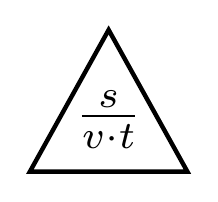
\begin{tikzpicture}[scale=2, every node/.style={scale=2}]
        \draw[ultra thick] (-0.5,-0.5) -- (0,-0.5) node[anchor=south, align=center] {\(\frac{s}{v \cdot t}\)} -- (0.5,-0.5) -- (0,0.4) -- cycle;
    \end{tikzpicture}
\end{figure*}

Denna kan användas genom att täcka för den sökta enheten med ett finger. och sedan kommer formel för den övertäcka enheten bli kvar. Sammanfattat gäller följande formler:
\begin{align*}
    s &= v \cdot t \\
    v &= \frac{s}{t} \\
    t &= \frac{s}{v} \\
\end{align*}

\section{Likformigt accelererande rörelse}
Om hastigheten inte längre är konstant är den enklaste nästa steg att accelerationen $a$ är konstant. då gäller följande formler:
\begin{align*}
    s &= \frac{at^2}{2} + v_0t + s_0 \\
    v &= at + v_0 
\end{align*}

\section{Allmän rörelse}
All rörelse kan beskrivas med hjälp av de ovanstående formlerna men man måste blanda in lite integral- och differentialkalkyl. För att uppnå denna fullständinga definition vill vi först tänka på rörelsens storheter som funktioner av tiden:
\begin{equation*}
    s(t) \text{ för sträcka, } v(t) \text{ för hastighet och } a(t) \text{ för accelration.}
\end{equation*}
Med detta kan vi sedan beräkna deras relation i alla möjliga fall. Här antar jag att du är bekant med tanken bakom integraler och derivator så här är snabbversionen av alla generella formler givet att $a(t)$ är linjärt:
\begin{align*}
    s(t) &= \frac{kt^3}{6} + \frac{a_0t^2}{2} + v_0t + s_0 \\
    v(t) &= \frac{kt^2}{2} + a_0t + v_0 \\
    a(t) &= kt + a_0
\end{align*}
eftersom
\begin{align*}
    v(t) &= s'(t) \\
    a(t) &= v'(t) = s''(t) \\
    s(t) &= \hyperref[def:indefint]{\int} {v(t)}\, dt = \iint{a(t)}\, dt\, dt
\end{align*}
(För fullständig härledning och teckenförklaring se bilaga \ref{derive:allmänrörelse}) Utifrån detta kan vi nu beräkna all rörelse bara vi vet formeln för en av storheterna. Om det inte finns en formel ska den hittas experimentellt eller så går det inte. Man kan sätta in valfri funktion för $a(t)$ och om man integrerar korrekt får man ändå rätt svar så detta är verkligen en allmän metod.

\section{Rörelsemängd}
Ett föremåls rörelsemängd är dess hastighet multiplicerat med dess massa och beteckans $p$. Formeln är: \[ p = mv\, \left[\mathrm{\frac{kg \cdot m}{s}  = kgm/s = N \cdot s}\right]\] Likt hastigheten är detta en vektor och har därför en riktning. Rörelsemängden skiljer sig från rörelseenergin $E_k$ eftersom $p \hyperref[def:propto]{\propto} v$ medan $E_k \propto v^2$.
\subsection{Stötar}
När två föremål krockar, dvs. stöter in i varandra så sker det ett utbyte av rörelsemängd. $p$ bevaras olika beroende på typen av stöt.
Se exempel nedan:
\begin{table*}[h]
    \centering
    \begin{tabular}{|c|c|c|}
        \hline
        Elastisk stöt          & Oelastiskt stöt             & fullständigt oelastisk stöt \\ \hline
        \begin{tikzpicture}
            \draw (0,0) -- (1,0);
        \end{tikzpicture}   &                             &                             \\ \hline
        Rörelseenergin bevaras & Rörelseenergin bevaras inte & Rörelseenergin bevaras inte \\ \hline
    \end{tabular}
\end{table*}
\subsubsection{Elastiskta stötar}
Vid s.k. \emph{elastiska stötar} så bevaras rörelseenergin. En elastisk stöt innebär att de två krockande föremålen inte fastnar i varandra utan förblir separata föremål. Generellt sett stöts de bort från varandra och åker åt olika håll efter stöten, dock inte alltid.

    \part{Krafter}
    En kraft är en vektorstorhet, dvs. att den har en riktning, som oftast definieras som produkten av accelerationen och massan.
    \begin{equation*}
        F=ma
    \end{equation*}
    Lägg märke till att vi inte använder vanlig vektornotation ($\vec{F}$) eftersom storleken av kraften är det man oftast söker, speciellt i denna kurs. Med detta menas att $F = |\vec{F}|$. Enheten för kraft är Newton (N) och beskrivs i grundenheter som $\frac{kg \cdot m}{s^2}$. När man söker riktningen av en kraft beskrivs detta nästan aldrig som en vektor ändå så denna fakta är mest för rätthet än nyttig användning.

    Det viktigaste som du kan veta om krafter är att enligt newtons lagar finns det alltid två av varje kraft. Han sade att ''varje kraft har en lika och motsatt \emph{reaktionskraft}'' (N III). Detta är exakt vad man tror det är. En kraft som verkar på ett föremål kommer att ha en reaktion från det föremålet i motsatt riktning med samma magnitud.

    Krafter kommer i många olika slag och de flesta från kursen finns förklarade nedan men en av de viktigaste och mest universella krafttyperna är normalkraften $N$ (mer sällsynt $F_n$). Denna är en kraft som är vinkelrät mot någon yta, dvs. normal mot ytan. Det finns enligt newtons tredje lag naturligtvis alltid två normalkrafter.
    \begin{exm}
        En låda sitter på ett bord under jordens gravitation. (I verkligheten är alla krafter i en och samma vertikala linje men är separerade för visualiseringens skull.)
        \begin{center}
            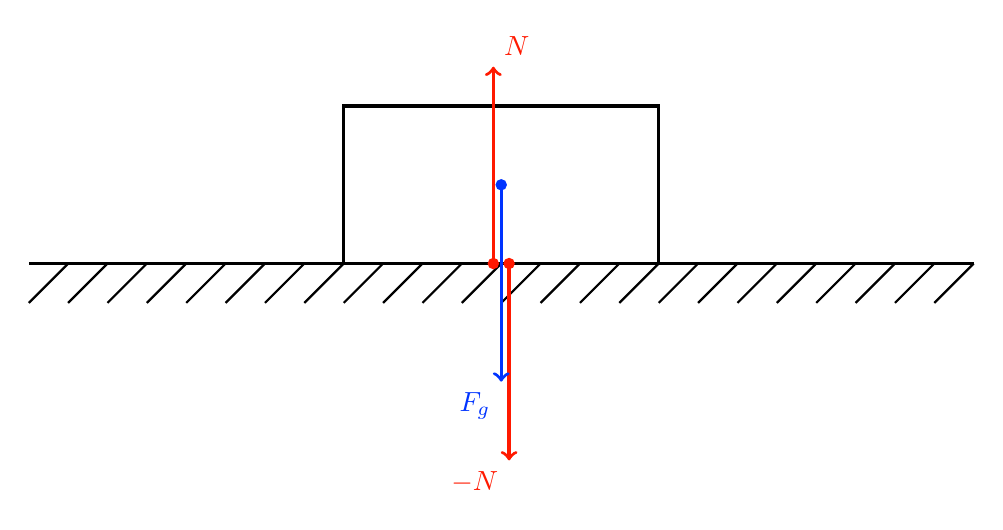
\begin{tikzpicture}
                \draw[thick] (-6,0) -- (6,0);
                \foreach \x in {-5.5,-5,...,6}  
                    \draw[thick] (\x,0) -- ++(-0.5,-0.5);
                \draw[very thick] (-2,2) rectangle (2,0);
                \draw[->, very thick, color=red!80!orange] (-0.1,0) -- ++(0,2.5) node [anchor=south west] {$N$};
                \filldraw[very thick, color=red!80!orange] (-0.1,0) circle [radius=0.05];
                \draw[->, very thick, color=red!80!orange] (0.1,0) -- ++(0,-2.5) node [anchor=north east] {$-N$};
                \filldraw[very thick, color=red!80!orange] (0.1,0) circle [radius=0.05];
                \draw[->, very thick, color=blue!80!cyan] (0,1) -- ++(0,-2.5) node [anchor=north east] {$F_g$};
                \filldraw[very thick, color=blue!80!cyan] (0,1) circle [radius=0.05];
            \end{tikzpicture}
        \end{center}
    \end{exm}

    \section{Tyngdkraften}
Tyngdkraften, bättre känd som gravitationen, är den kraft som två massor utgör på varandra enligt fysikens lagar. Den betecknas $F_g$ och har samma enhet som alla andra krafter. Formeln för tyngdkraften är följande:
\begin{equation*}
    F_g = G \cdot \frac{m_1m_2}{r^2}
\end{equation*}
$G$ är \emph{gravitationskonstanten} och har ett värde på $G \approx 6.67 \cdot 10^{-11}$, $m_1$ och $m_2$ är massorna av de två interagerande föremålen och $r$ är avstånden mellan deras masscentrum. Detta samband innebär att $F_g \hyperref[def:propto]{\propto} \frac{1}{r^2}$ vilket gör att tyngdkraft avtar myhcket snabbt när avståndet ökar.

\section{Friktionskraft}
Friktionskraften är den kraft som två föremål utgör på varandra när de är i kontakt och en yttre kraft verkar på ena föremålet medan en lika stor kraft inte verkar på det andra. Denna har beteckningen $F_f$ och har formeln
\begin{equation*}
    F_f = \mu N
\end{equation*}
där $\mu$ är det så kallade \emph{friktionstalet} eller \emph{friktionskoefficienten} och $N$ är normalkraften. Detta medför bland annat att $F_f \hyperref[def:propto]{\propto} N$ med en konstant faktor $\mu$. Vissa tycker att det är intuitivit att fritktionskraften skulle öka när kontaktytan ökar, men det gör den inte. Tänk på tryck, har vi samma normalkraft kommer trycker minska om arean ökar och vice versa, därmed ingen förändring i friktionskraft.

Det finns två typer av friktion: \emph{statisk-/vilofriktion} och \emph{glidfriktion}. Dessa är ganska självklara; vilofriktion är den maximala friktionskraften som kan uppstå när föremålet är stilla jämfört med sitt underlag och glidfriktion är den maximala kraften som kan uppstå när föremålet rör på sig gentemot sitt underlag. Båda kan beräknas enliga vanliga kraftresonemang givet att föremålet befinner sig i vila (den totala kraftresultanten är 0).

\section{Tryck}
Tryck är ett mått på hur kraft fördelar sig på en ytan. Tryck ($p$) mäts i Pascal (Pa) då $1\,\mathrm{Pa} = 1 \, \mathrm{N} / \mathrm{m^2}$ och beskrivs av följande formel:
\begin{equation*}
    p = \frac{F}{A} \, \left[\frac{\mathrm{N}}{\mathrm{m^2}} = \mathrm{Pa}\right]
\end{equation*}
Denna storhet existerar för att det inte alltid är det mest användbara att tala om enbart kraften. Skörheten av material beror exempelvis på tryck istället för enbart kraft. Du kan trycka med flera MN totalt på ett föremål och så länge arean är stor nog kommer varje individuella punkte enbart uppleva en mycket liten del av kraften.

\section{Lyftkraft \& Arkimedes princip}
Lyftkraft ($F_L$) är den kraften som verkar uppåt på ett föremål som är nedsänkt i en vätska eller ideal gas. Med ideal gas menas en gas som följer ideala gaslagen ($PV=nRT$). I dessa förhållanden säger arkimedes princip att kraften som verkar uppåt kommer att vara lika med tyngden av den vätska som ''puttas undan'' av det nedsänkta föremålet.
\begin{exm}
    Betrakta en fisk som sänks ned i vattnet. Den kommer då uppleva både tyngd- och lyftkraft. Det kommer visa sig att om fiskens densitet är lika med vattnets (föreställ dig en fisk av vatten) kommer den att just precis flyta. Vi vet att volymen av det undanputtade vattnet är precis lika med fiskens volym. Vi vet även att fiskens och vattnets densitet är densamma vilket medför att deras tyngd är och konstant. I slutändan leder detta till att $F_L$ och $F_g$ tar ut varandra.
    \begin{center}
        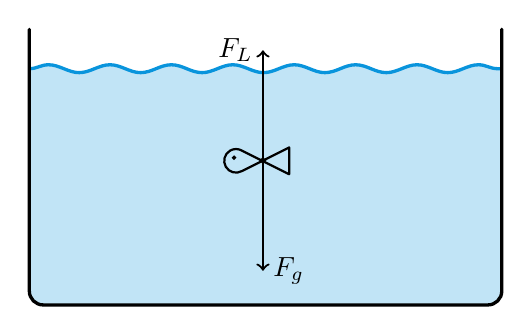
\begin{tikzpicture}[every path/.style={thick}]
            %water
            \draw[very thick, decorate, decoration={snake,amplitude=.5mm,segment length=0.78cm, post length=.1mm}, color=cyan!80!blue] (-3,-0.5) -- ++(6,0);
            \fill [color=cyan!80!blue, fill opacity=0.25] decorate [decoration={snake,amplitude=.5mm,segment length=0.78cm, post length=.1mm}] {(-3,-0.5) -- ++(6,0)} [rounded corners=5pt] -- ++(0,-3)  -- ++(-6,0) -- ++(0,3);
            %border
            \draw[very thick, rounded corners=5pt, line cap=round] (-3,0) -- ++(0,-3.5) -- ++(6,0) -- ++(0,3.5);
            %fish
            \draw[line join=round] (0.3,-1.5) -- ++(-0.6,-0.3) arc [start angle=300, end angle=60, radius=0.15cm] -- ++(0.6,-0.3) -- cycle;
            \filldraw (-0.4, -1.63) circle [radius=0.3pt];
            %forces
            \filldraw (-0.033,-1.666) circle [radius=.7pt];
            \draw[->] (-0.033,-1.666) -- ++(0,1.4) node [anchor=east] {$F_L$};
            \draw[->] (-0.033,-1.666) -- ++(0,-1.4) node [anchor=west] {$F_g$};
        \end{tikzpicture}
    \end{center}
\end{exm}
I mer generella fall behöver man dra algebraiska slutsatser. En härledning för arkimedes princip hittar du i bilaga \ref{def:arkimedes}. I praktiken är det dock enbart tre samband du bör kunna:
\begin{align*}
    \rho_{\textit{föremål}} > \rho_{\textit{vätska}} &\implies F_g > F_L \implies \text{den sjunker} \\
    \rho_{\textit{föremål}} < \rho_{\textit{vätska}} &\implies F_g < F_L \implies \text{den lyfter} \\
    \rho_{\textit{föremål}} = \rho_{\textit{vätska}} &\implies F_g = F_L \implies \text{inget händer} 
\end{align*}
Utöver dessa bör du även kunna den generella formeln för lyftkraft:
\begin{equation*}
    \tcboxmath{F_L = \rho_{\textit{vätska}} \cdot g \cdot V_{\textit{föremål}} \, \left[\mathrm{N}\right]}
\end{equation*}
Vi vet ju att $\rho V = m$ och vi vet att $mg=F_g$ alltså vi att $F_L$ motsvarar tyngden av den undanträngda vätskan.

    \newpage
    \appendix
    \section{Härledningar}
    \label{appendix:härledning}
    \subsection{Teckenförklaring}
I denna sammanfattning använder jag vissa matematiska tecken som är ibland mer advancerade än bara de vi går igenom. Följande är deras definitioner:

\subsubsection*{Indefinit integral}
\label{def:indefint}
Tecknet $\int$ står för en \emph{indefinit integreal} när inga integrationsgränser är angivna. Detta motsvarar att hitta primitiv funktion till något så givet att \[f(x) = kx + m\] gäller att
\begin{equation*}
    F(x) = \int{f(x)}\, dx = \frac{kx^2}{2} + mx + C
\end{equation*}

Detta gäller för alla funktioner oavsett variabel, grad eller liknande man använder helt enkelt vanliga primitiva funktionsregler på lite mer effektivt sätt. Ja, man kan använda indefinit integral på prov enligt Mattias.

\subsubsection*{Proportionalitetstecken}
\label{def:propto}
Proportionalitetstecknet $\propto$ används för att visa att en variabel är proportionell mot någon annan variabel eller något uttryck. Givet proportionaliteten $y=kx$ kommer det se ut som \[y \propto x \text{ med en faktor k}\] 

\subsection{Allmän rörelse}
\label{derive:allmänrörelse}
Givet att funktionen $a(t) = kt + a_0$ där $a_0$ är en konstant startacceleration kommer nu härledningen till $s(t)$ från detta:
\begin{gather*}
    \begin{aligned}
        \centering
        a(t) &= kt + a_0 \\
        v(t) &= \int{a(t)}\, dt = \frac{kt^2}{2} + a_0t + C_1 & C_1 &= v_0 \\
        v(t) &= \frac{kt^2}{2} + a_0t + v_0 \\
        s(t) &= \int{v(t)}\, dt = \frac{kt^3}{6} + \frac{a_0t^2}{2} + v_0t + C_2 & C_2 &= s_0
    \end{aligned} \\
    \tcboxmath{s(t) = \frac{kt^3}{6} + \frac{a_0t^2}{2} + v_0t + s_0}
\end{gather*}
\noindent Här är \(a_0 = \text{acceleration från start, } v_0 = \text{hastighet från start och } s_0 = \text{den redan färdade sträckan från start}\). Alla integraler kan beräknas med reglerna från formelsamlingen.

\subsection{Lagen om rörelsemängdens bevarande}
\label{derive:conserverationmomentum}
Denna lag ger oss att efter en stöt kommer rörelsemängden i systemet alltid att bevaras. Föreställ dig att två föremål med massam $m_1$ och $m_2$ har hastigheterna $u_1$ och $u_2$. De krockar sedan elastiskt där föremål 1 verkar på föremål 2 med kraften $F_1$ medan föremål 2 verkar med kraften $F_2$. Sambandet mellan dessa krafter är
\begin{equation*}
    F_2 = -F_1 \: \text{enligt N III}
\end{equation*}
Föremålens krock pågår under en liten tid $\Delta t$. Impulsen som de båda påverkar varandra med blir då:
\begin{align*}
    \Delta p_1 &= F_2 \cdot \Delta t = m_1v_1 - m_1u_1 \\
    \Delta p_2 &= F_1 \cdot \Delta t = m_2v_2 - m_2u_2
\end{align*}
där $v_1$ och $v_2$ är hastigheterna efter krocken. Givet ovanstående kraftsamband får vi då:
\begin{align*}
    \Delta p_1 = -F_1 \cdot \Delta t &= -(F_1 \cdot \Delta t) = -\Delta p_2 \\
    \Delta p_1 &= -\Delta p_2 \\
    m_1v_1 - m_1u_1 &= -(m_2v_2 - m_2u_2) \\
    m_1v_1 - m_1u_1 &= -m_2v_2 + m_2u_2 \\
    m_1u_1 + m_2u_2 &= m_1v_1 + m_2v_2 \\
    p_{innan} &= p_{efter} \qed
\end{align*}
alltså konserveras rörelsemängden.

\subsection{Arkimedes princip}
\label{def:arkimedes}
Här följer en härledning för ett föremål med godtycklig volym och densitet givet arkimedes princip. Utifrån bilden kan vi se ett föremål med oregelbunden form som är ett vanligt prisma. Utifrån detta vet vi att $V = Ah$. Vi vet även den generella formeln för tryck i vätska: $P = \rho gh$. I detta fall är $h$ djupet i vätskan, jag vet att det är förvirrande med två $h$ men hellre detta än icke-standardiserade variabler. Detta ger oss följande iakttaglser:
\begin{equation*}
    P_1 = \rho gd \qquad P_2 = \rho g(d+h)
\end{equation*}
Efter detta inser man även att
\begin{equation*}
    |d+h| > |d| \implies P_2 > P_1
\end{equation*}
Vill vi få ut kraft ur ett tryck får vi att $F = PA$. Detta leder oss då till följande:
\begin{equation*}
    F_1 = P_1A \qquad F_2 = P_2A
\end{equation*}
sedan vet vi att
\begin{equation*}
    P_2 > P_1 \implies F_2 > F_1
\end{equation*}
För tydlighetens skulle är $F_2$ kraften som verkar uppåt på botten av föremålet på grund av vätsketrycket och $F_1$ är kraften som verkar nedåt på toppen av föremålet på grund av vätsketrycket. Utifrån dett kan vi logiskt inse att
\begin{gather*}
    \begin{aligned}
        F_L &= F_2 - F_1 \\
        F_L &= P_2A - P_1A \\
        F_L &= A(\rho g(d+h)) - A(\rho gd) \\
        F_L &= A\rho g((\cancel{d}+h)-\cancel{d}) \\
        F_L &= A\rho gh = Ah \cdot \rho g \qquad Ah = V
    \end{aligned} \\
    \tcboxmath{F_L = \rho gV \qed}
\end{gather*}
\begin{center}
    \begin{tikzpicture}[every path/.style={very thick}]
        %container
        \filldraw[color=cyan!80!blue, fill opacity=0.25] decorate [decoration={snake,amplitude=0.6mm,segment length=0.79cm}] {(-7,-0.3) -- ++ (14,0)} [rounded corners=5pt] -- ++(0,-6.7) -- ++(-14,0) [sharp corners] -- cycle;
        \draw[ultra thick, rounded corners=5pt, line cap=round] (-7,0) -- ++(0,-7) -- ++(14,0) -- ++(0,7);
        %shape
        \draw[line join=round] (-1,-1.5) .. controls (-0.8, -2) and (-0.4, -1.4) .. (0,-1.5) arc [start angle=85,delta angle=-200, radius=0.3cm] node [pos=0.4, anchor=east] {$A$} .. controls (-0.5,-1.9) .. (-1.3,-1.85) arc [start angle=272, delta angle=-250, radius=0.3cm] -- cycle;
        \draw[line join=round,yshift=-1.7cm] (-1,-1.5) .. controls (-0.8, -2) and (-0.4, -1.4) .. (0,-1.5) arc [start angle=85,delta angle=-200, radius=0.3cm] node [pos=0.4, anchor=east] {$A$} .. controls (-0.5,-1.9) .. (-1.3,-1.85) arc [start angle=272, delta angle=-250, radius=0.3cm] -- cycle;
        \draw[dashed, line cap=round] (-1.61,-1.5) -- ++(0,-1.7);
        \draw[dashed, line cap=round] (0.27, -1.8) -- ++(0,-1.7);
        %height
        \draw[decorate, decoration={calligraphic brace,amplitude=2mm}, xshift=0.1cm] (0.27, -1.8) -- ++(0,-1.7) node[pos=0.5, anchor=west, right=2pt] {$h$};
        \draw[decorate, decoration={calligraphic brace,amplitude=2mm}, xshift=0.1cm] (0.27, -0.23) -- ++(0,-1.53) node[pos=0.5, anchor=west, right=2pt] {$d$};
    \end{tikzpicture}
\end{center}

    \section{Exempel}
    \label{appendix:exempel}
\end{document}